\documentclass[authoryear,preprint,review,12pt]{elsarticle}

%\usepackage[utf8]{inputenc}
\usepackage{amsmath}
\usepackage{amssymb}
\usepackage{hyperref}
\usepackage{multirow}
\usepackage{defs}
\usepackage{lineno}
\usepackage{rotating} % For sideways figure

\journal{Renewable Energy}

\begin{document}

% Front page ----------------------------------------------------------------------
\begin{frontmatter}

\title{A Scalable Wave Resource Assessment Methodology: Application to U.S. Waters}

\author[a1]{Levi Kilcher\corref{cor1}}
\ead{levi.kilcher@nrel.gov}
\cortext[cor1]{Corresponding Author}

\author[a2]{Gabriel Garc\'ia Medina}
\author[a2,a3]{Zhaoqing Yang}

\affiliation[a1]{organization={National Renewable Energy Laboratory},
                  addressline={15013 Denver W Pkwy},
                  city={Golden},
                  postcode={80401},
                  state={CO},
                  country={United States}}
\affiliation[a2]{organization={Coastal Sciences Division, Pacific Northwest National Laboratory},
                 addressline={1100 Dexter Ave N, Ste 500},
                 city={Seattle},
                 postcode={98109},
                 state={WA},
                 country={United States}}
\affiliation[a3]{organization={Department of Civil and Environmental Engineering, University of Washington},
                 city={Seattle},
                 postcode={98195},
                 state={WA},
                 country={United States}}

\begin{abstract}
Waves deliver massive quantities of energy to populated coastlines around the world, and wave energy technology research and development has accelerated over the last two decades. Throughout this time national and regional resource assessments have utilized disparate methodologies, which can cause confusion and skepticism. In this work we describe a theoretical wave resource assessment methodology that addresses many of the major areas of inconsistency and debate. Applying this revised methodology to U.S. waters, we find the U.S. wave energy resource to be 3300 – 4100 TWh/yr, with region totals of: 2000 – 2500 TWh/yr in Alaska, 510 – 630 TWh/yr along the U.S. west coast, 380 – 470 TWh/yr along the east coast, 70 TWh/yr in the Gulf of Mexico, and 18-33 TWh/yr in Puerto Rico and the U.S. Virgin Islands.
\end{abstract}

%%Graphical abstract
% \begin{graphicalabstract}
% \includegraphics{grabs}
% \end{graphicalabstract}

%%Research highlights
\begin{highlights}
\item Novel, scalable methodology for theoretical wave resource assessment
\item Updated wave resource assessment for U.S. Exclusive Economic Zone
\item Addresses main shortcomings of previous national wave resource assessments
\end{highlights}

\begin{keyword}
    Wave resource assessment \sep wave hindcast \sep scalable methodology
\end{keyword}

\end{frontmatter}

% Main Text --------------------------------------------------------------
\begin{linenumbers}
\section{Introduction}

Though wave energy technology is still at an
early-stage of technology development, interest in wave energy has grown considerably over the last decade
\citep[]{babaritOceanWaveEnergy2017}. For example, the Ocean Energy Systems executive committee has set a goal of 300GW of installed ocean energy capacity by 2050 \citep[]{huckerbyInternationalVisionOcean2017}. Wave energy is seen as particularly
valuable for its predictability and reliability on timescales of hours
to a few days \citep{parkinsonIntegratingOceanWave2015}, and for the
fact that the resource is concentrated along coastlines where large
fractions of the world's populations live. Furthermore, the
U.S. Department of Energy (DOE) has launched the ``Powering the Blue
Economy'' initiative designed to support the development of
technologies that provide power to unique market applications such as
desalination, ocean sensing, aquaculture, maritime shipping, and coastal community
resiliency \citep{livecchiPoweringBlueEconomy2019}. 

There have been several notable wave resource assessments over the last two decades that have consistently improved the accuracy and spatial coverage of our understanding of the U.S. wave energy opportunity \citep[]{EPRIwaveresource2011, bedardOceanWaveEnergy2005, allahdadiDevelopmentValidationRegionalscale2019, garciamedinaWaveResourceCharacterization2021, yangCharacteristicsVariabilityNearshore2020, liWaveEnergyResources2021}.
Throughout this time there have been ongoing discussions about how best to quantify and describe wave energy opportunities (i.e., the physical energy contained in the resource). 

This work has led to important definitions of terms such as ``theoretical resource'', ``technical resource'' and ``practical resource'' \citep[]{internationalelectrotechnicalcommissionPartTerminologyEdition2020}. There is also a distinction between: a) {\em site}-focused resource assessments, which provide the data (time-series of wave energy, wave height, wave period, wave direction, etc.) that project developers need for identifying sites and planning projects \citep[e.g., ][]{internationalelectrotechnicalcommissionPart101Wave2015, robertsonCharacterizingShoreWave2014, kumarWaveEnergyResource2015}, and b) {\em regional} resource assessments, which quantify the total wave energy resource across a large section of coastline (i.e., averaged in time and space to get a single number) that the public, policy makers, and other stakeholders use to quantify the high-level value proposition \citep[e.g., ][]{EPRIwaveresource2011, gunnQuantifyingGlobalWave2012, hemerRevisedAssessmentAustralia2017}.

The International Electrotechnical Commission's Technical Committee on
Marine Energy (IEC TC114) has published a robust and consensus-based methodology for wave resource for wave resource {\em site}-assessment \citep[][hereafter, 62600-101]{internationalelectrotechnicalcommissionPart101Wave2015}. That work does not, however, provide definitive guidance on how to aggregate the results into a regional total. Lacking a definitive consensus-based methodology, {\em regional} wave resource assessments have utilized disparate methodologies, which can lead to skepticism and confusion.

Several assessments, including the most recent U.S. benchmark study, have estimated total theoretical resource by integrating omni-directional wave power along the length of a selected contour \citep[]{}. However, as the national academy points out...



This work seeks to establish a definitive wave resource assessment methodology 

resolve outstanding questions associated with regional theoretical resource assessment by proposing a methodology that 

followed the benchmark U.S. resource assessment study the total U.S. wave resource -- which was published prior to 62600-101 -- has provided the first com-prehensive estimate of the nation’s wave energy resource, and has been an im-portant reference for motivating private and public investment in wave energyresearch ever since (Jacobson et al., 2011, hereafter ‘EPRI 2011’).  A few yearslater, the International Electrotechnical Commission’s Technical Committee onMarine Energy (TC114) published a wave resource assessment technical specifi-cation (International Electrotechnical Commission, 2015, hereafter, 62600-101),that  provides  a  consensus-based  methodology  for  wave  resource  for  wave  resource site-assessment.

Some works follow the EPRI 2011 methodology, while others do account for directionality, but most assessments at large scales avoid the issue resulting in a reconnaissance-level assessment that does not directly quantify total power available across the region. This makes it difficult to make apples-to-apples comparisons, puts the industry’s credibility at risk, and does not provide policy makers with the kind of information they need. 

which can lead to skepticism and confusion \citep[]{internationalelectrotechnicalcommissionPart101Wave2015, robertsonCharacterizingShoreWave2014, gunnQuantifyingGlobalWave2012, hughesNationalscaleWaveEnergy2010, hemerRevisedAssessmentAustralia2017, nationalresearchcouncilEvaluationDepartmentEnergy2013}.

The 2013 National Academy of Sciences (NAS) review of U.S. marine energy resource assessments found that in general the resource assessments provide “a useful contribution to understanding the distribution and possible magnitude of marine and hydrokinetic energy sources in the United States,” but also detailed several specific technical critiques. In the case of wave energy, the NAS review stated that because the method used did not account for wave direction, it “has the potential to double-count a portion of the wave energy”. 

Furthermore, discussions with several leading wave energy experts revealed two additional key criticisms of existing wave resource assessment methods: 1) that the domain of the resource assessments are often arbitrary and are not necessarily consistent with relevant political boundaries, and 2) that the methods only account for wave energy arriving at the edge of the boundary and not for waves generated within the boundary.

These lingering critiques have resulted in a “define your own method” approach to regional wave resource assessment. 

The primary objective of this work is to address the critiques and questions in the previous paragraph directly, and thereby bring clarity to the topic of region-scale theoretical resource assessment. In time, we hope that this clarity serves as a basis for consensus on the subject so that researchers can deliver assessments that are consistent, and then move on to other important research areas – including technical and practical resource assessment. The secondary objective of this work is to provide a refined estimate of the U.S. wave resource based on this new method and updated model outputs.

%%% Local Variables:
%%% TeX-master: "wave_res"
%%% End:

\section{Background}
% The majority of this section can probably be removed/tightened and added to the intro?

Ocean surface waves are generated by wind blowing across the ocean surface. The
energy is transferred from the atmosphere to the ocean by the friction of wind
on the ocean surface, and by pressure differentials associated with the wind
blowing across the wave crests
\citep[]{phillipsDynamicsUpperOcean1980,youngWindGeneratedOcean1999}. At the
site of wave generation - in a storm, for example - waves of many frequencies,
$f$, are generated. As these waves propagate across the ocean surface they cross
paths with waves from other locations. Thus, at any point on the ocean surface,
the sea-state is composed of a mix of waves of differing frequencies, coming
from different directions, and originating at different points in time and
space. The distribution of wave energy at any point is therefore quantified as a function of 
frequency (or period) and direction 
(Figure \ref{fig:dirspec}), hereafter the `direcitonal spectrum'.

Regional wave resource assessments are typically accomplished using spectral
wave energy simulations. These models simulate wave energy propagation according
to wave energy kinematics (i.e., at the group velocity), and they contain
‘source and sink’ terms to estimate the generation, evolution (i.e., non-linear
interactions that transfer energy between frequencies), and dissipation of
spectral wave energy in space and time (Booij et al. 1999; The WAVEWATCH III
Development Group (...). These terms are based on empirical measurements, and
are typically functions of the wind forcing and bathymetry (both of which must
be supplied as input to the model).

There is broad consensus that these models should: utilize modern physics packages (source and sink terms), span several decades to account for inter-annual variability, and be validated against several measurement points in the region of interest. While there is consensus and agreement on these points, there has been considerable confusion regarding how to use the model data to compute resource totals. This confusion has three primary sources:


\begin{figure}[ht]
  \centering
  \includegraphics[width=0.9\linewidth]{../fig/dirspec.png}
  \caption{Directional spectrum}
  \label{fig:dirspec}
\end{figure}

\begin{enumerate}
\item Waves can come from multiple directions at the same time, and many WEC types can absorb energy equally from all directions. How does one reconcile this detail of individual devices with the need to account for wave-flux directionality when computing a line-integral in a regional assessment?
\item Local winds can generate energy inshore of the selected contour. How does one account for that energy? This issue is confounded by the fact that source-terms are proportional to the wave spectrum (wave size).
\item Wave models are typically configured to propagate wave energy throughout the domain (not absorb at the chosen boundary). How does one know whether or not wave energy crossing the boundary has already been ‘counted’ at a different location and time?
\end{enumerate}

Each of the above issues are considered in more detail in the following subsections.

\subsection{Wave directionality}

\begin{figure}[ht]
  \centering
  \includegraphics[width=0.7\linewidth]{../diagram/Dot-Product_Schematic01}
  \caption{A schematic depicting the importance of directionality in computing energy-flux totals. The upper and lower sequence of pictures depict the same wave (left) encountering a contour at different angles (middle). The red-arrow depicts the wave direction, and the black arrow the contour-normal. The angle between these vectors is $\theta$ (right).}
  \label{fig:directionality}
\end{figure}

Because wave energy flux is a vector (directional) quantity, it’s sum must be computed using a method that properly accounts for the directionality. Figure 3 illustrates this point: in both the top and bottom rows, the total wave energy flux in the 1 km wide wave is 1 MW. If, however, the wave-direction is unknown and one were to naively multiply the wave-flux magnitude by the length of the contour (i.e., incorrectly assume that the wave flux is perpendicular to the contour), the lower example will overestimate the resource by a factor of 3. Thus it is important to utilize a ‘dot-product’ when computing wave-flux totals. When waves from different directions are arriving at a location simultaneously, the dot-product should be computed for each wave crossing the contour, and then these totals summed separately.

However, in order to reduce the data-storage burden, wave models are often configured to store summarized (incomplete) information. This may mean that no directional information is preserved in the model output (e.g., only wave height and period is available), or perhaps only the ‘average wave direction’ or the ‘direction of the largest wave’ are available. Resource assessments based on these kinds of data will contain errors due to incorrectly accounting for wave direction. The magnitude and sign of this error depends on the details of the data limitations, and the assumptions that are made to accommodate these limitations.

An earlier U.S. wave resource assessment suggested that directionality could be ignored because many WECs (e.g., a ‘point absorber’) can absorb energy equally from any direction (Jacobson, Hagerman, and Scott 2011). While this reasoning is true for a single device, it breaks down when considering an array of devices that are close enough together to capture all of the incident resource. It is, after all, the purpose of resource assessment to estimate the total available resource.

In particular, when the devices are packed close enough together to capture all incoming wave energy, some devices - for certain wave directions - will be wholly or partially in the ’shadow’ of others. The shadowed (i.e., ‘down wave’) devices will not be subjected to the full resource intensity because the shadowing (‘up wave’) devices will have captured some fraction of the incident resource (Babarit 2013). The details of which devices are shadowed vs. shadowing depends on the details of the array layout and the incident wave direction. But this is entirely the point: wave directionality is as important for tightly-spaced arrays of point absorbers as it is for directional device types. For the purposes of - and at the scale of - regional resource assessment, we can ignore the details of device type and array configuration and instead treat the “array” as a line that absorbs all incoming wave energy (i.e., using a dot-product).

We use a one-way dot-product to compute wave energy flux 'into' the box \citep[]{gunnQuantifyingGlobalWave2012}. 
% What is the right amount to discuss the 'directional method' issue? Reference the EPRI 2011 RA, and the NAS Review? Then, ...

\subsection{Local Resource}

To our knowledge, all prior wave resource assessments have been completed by considering the remote resource only. That is, by estimating wave-energy flux across a boundary that is selected to be representative of the coastline of interest. This approach has raised the question: what about waves that are generated inshore of the chosen boundary (hereafter, the ‘locally generated energy’)? The answer has usually been that this contribution is believed to be small, but few have undertaken the task of quantifying it.

The rationale for neglecting the locally generated energy seems to have been based on some combination of: a) it can’t be calculated from the data I have, b) the ocean surface inshore of the contour I’ve selected is very small compared to the rest of the ocean (so the local energy should be small compared to the remote energy), and c) the local generation is likely to be dominated by relatively short-period waves, which are lower energy (per wave height). While this reasoning is reasonable for the first generation of wave resource assessments, we think it is time to consider this term explicitly in wave resource assessments.

We configure our WW3 model to write-out the wind-input and dissipation source terms for the entire domain of interest. These terms have units of power unit-crest-length, per unit fetch-length (e.g., W/m2). Thus, an area integral of these terms - over the region of interest - provides an estimate of the rate of energy input from the wind to the water. Adding these terms to the wave resource budget has three details worth noting, described in the following subsections.

\subsubsection{Source-term directionality}

First, we point out that - while the source terms are directional - this directionality is unimportant for the purposes of resource assessment. This may be surprising to the reader, considering the importance we have attributed to the directionality of the ‘remote’ resource, but we point out that this is an entirely different term involving an area-integral rather than a line integral. In the case of the line-integral, wave directionality was important relative to the boundary line (edge of the array of devices). Now, inside the boundary, we presume for the purposes of resource assessment that devices essentially ‘blanket’ the ocean so that wave energy can be extracted as soon as it is created. Within the boundary, as wave energy is added to the wave field, the directionality of that energy is unimportant to calculating the total there are devices in all directions.

To put the above in the terms of control volume mathematics (two-dimensional): the rate of change of a quantity (e.g., energy) inside a boundary is equal to the line-integral of the flux across the boundary, plus the area-integral of the sources (and sinks) of that quantity across the entire volume. This is exactly what we’re doing here, we’re adding a line-integral of fluxes and an area integral of source-terms to get a total.

\subsubsection{Source-term non-linearity}

Second, the magnitude of the input source term is proportional to the amplitude of the wave energy spectrum. That is, larger waves grow faster than small ones (i.e., wave growth is non-linear). This is a fundamental concept of wave growth, but it complicates the task of calculating the ‘locally generated energy’. The simplest scenario would be to run a “lake” simulation, in which the simulation is configured so that no remote wave-flux crosses into the study-area (i.e., it is all absorbed at the boundary). Then one simply lets the local waves build within the study-area based solely on local generation, and calculate that total power.

In this simplistic approach, we are imagining a scenario in which all ‘remote’ wave energy is absorbed at the offshore boundary of the study-area. However, one wonders if it would be better to allow the waves to propagate into the study-area so as to increase the magnitude of the source terms (which will be larger for these larger waves). Furthermore, because the source terms are proportional to the wave-spectrum, the frequency dependence of the source terms is also highly dependent on the wave-field. This makes calculating the source-term resource particularly challenging if one plans to weight frequency bands differently (e.g., ignore very-high and very-low frequency bands). In this work we do not weight frequency bands differently.

For the purposes of RA, this essentially becomes an optimization problem of ‘where and when’ to extract energy to maximize total extractable power (i.e., maximize source-term wave growth relative to dissipation terms). From a purely energetics standpoint (neglecting the frequency content of the waves, and the frequency dependence of wave converters), wave energy would ideally be extracted just ‘down-wave’ from a location where winds have added energy to the wave-field (i.e., before dissipation begins to reduce the total wave energy). However, because storms move around the practicality of harvesting wave energy just downstream of generation sites (storms) is probably unrealistic.

From a practical standpoint, these details are relatively unimportant until we actually possess the technology to extract wave energy on large scales. Rather than optimizing power extraction siting, we can estimate the range of source terms by assuming that the ‘lake’ simulation provides a lower-bound estimate of the source terms, and that a simulation with the full remote waves present inside the study-area provides an upper-bound estimate of the source terms.

\subsubsection{Source-term accuracy}

Finally, there is considerable debate on the topic of the accuracy of the formulation of the source terms, and new source term formulations are frequently being proposed. In this work, we use the ST4 package because... And, we assess the uncertainty in source terms by looking at the differing magntiudes of the terms with/without remote wave energy. Some authors have shown that while the magnitude of the sum of the input and dissipation terms seems reasonable, the values of these terms individually may have larger error (Moghimi et al. 2016). This means that, until we have more confidence in the values of these terms, results based on them should be carefully considered...

To summarize, we believe that considering the source terms is an important step toward a more comprehensive wave resource assessment. And, while there are still outstanding issues to be investigated (namely: the importance of source-term non-linearity and accuracy), estimating the uncertainty in these terms is useful for a more complete picture of the wave resource uncertainty as a whole.

\subsection{Has this wave been counted?}

\begin{figure}[ht]
  \centering
  \includegraphics[width=\linewidth]{../diagram/schematic03.png}
  \caption{A schematic of wave energy flux crossing a contour for the scenarios depicted by arrows A, B, C, D, E. The diagram depicts three distinct methods for summation: ‘traditional’ (pink), ‘bi-directional’ (orange), and ‘one-way’ (cyan). At each arrow intersection, the ‘+’ or ‘-’ indicates whether that method adds to or subtracts from the total depending on the direction relative to the contour (upper left legend). At the end of each arrow, the total sum for each method is indicated (ideally each wave should be counted ‘1’ time). The table at lower-right summarizes these totals.}
  \label{fig:wave-counting}
\end{figure}

The third source of confusion in calculating wave resource totals is perhaps best summarized by the question: “Has this wave been counted already?” This issue is related to the details of the use of the dot-product (a.k.a., ‘scalar product’) for calculating wave resource totals. The ‘traditional’ dot-product of two vectors a and b is:

\begin{align}
  \vec{a} \cdot \vec{b} = a b \cos(\theta)
\end{align}

Where $a$ and $b$ are the magnitudes of the vectors $\vec{a}$ and $\vec{b}$, respectively, and $\theta$ is the angle between them. This equation properly accounts for the wave energy that propagates across the contour and is eventually dissipated on the coastline (Figure \ref{fig:wave-counting}, arrow A). It also works for waves that cross a boundary an odd number of times on their way toward the coastline (e.g., arrows B and D). However, waves that cross the boundary an even number of times are not counted at all (arrow C, traditional total of 0), and waves that cross the boundary in the ‘outward’ direction are subtracted from the total (arrow E, traditional total of -1), both of which are not the desired result.

This problem arises from the fact that there is no way to know whether wave energy crossing at one location has already been counted at a different location. The traditional dot-product calculates a ‘net’ flux into the box, but it does not include the wave energy that passes through the region or originates within it (both of which could be captured by devices inside the region).

For example, if wave energy propagates past an island, it might pass into and then out of the study-area. At the point where it passes in, the energy in the wave will be added to the total, but it will be subtracted again where it passes back out of the resource area. Thus, using the traditional dot-product method, this wave-group will not be counted in the resource total. To address this issue, many wave resource assessments have used a ‘one-way’ dot product:

\begin{align} \label{eqn:oneway}
\begin{split}
  \vec{a} \cdot \vec{b} & = ab \cos(\theta) \qquad \mathrm{for} |\theta| < 90 \degrees\\
      & = 0 \qquad \mathrm{otherwise}
  \end{split}
\end{align}

This approach adds wave energy when it fluxes into the domain ($|\theta| < 90\degrees$), and does not count wave energy that fluxes out of the domain ($|\theta| > 90\degrees$). Therefore, the one-way method accurately quantifies wave energy that fluxes into the domain and dissipates on the coastline (Figure \ref{fig:wave-counting}, arrow A), and wave energy that propagates into and then out of the domain (arrow C), but it ‘double counts’ wave energy that propagates into and out of the domain more than once (arrows B and D). Finally, it does not include the local resource that fluxes out of the domain (arrow E). This allows us to add the local resource separately, as outlined in the previous subsection.

We are therefore left with two results of the line-integral summation:
\begin{enumerate}
\item The traditional dot-product gives an underestimate of the total resource (because wave energy that fluxes out of the domain is subtracted from the total), and
\item The one-way dot product, when added to the local resource estimate, will give an overestimate of the total resource.
\end{enumerate}

\section{Method}

The overarching goal of this study is to define the wave energy resources and to
develop a consistent and accurate methodology to estimate the total
theoretically available wave resource for a given region. The wave climate is
simulated by implementing WAVEWATCH III® v5.16
\citep{tolmanDistributedmemoryConceptsWave2002} in all model
simulations in this study. WAVEWATCH III® (hereafter WW3) is a skillful and well
established numerical model that has been implemented successfully in many
previous wave resource assessments
\citep[e.g.,][]{garcia-medinaWaveResourceAssessment2014,yangWaveModelTest2017}.
WW3 solves the five-dimensional action balance equation:

\begin{align}
    \frac{DN}{Dt} = \frac{\Src{tot}}{\sigma} = \frac{1}{\sigma}\left ( \Src{in} + \Src{ds} + \Src{nl} + \Src{bot} + \Src{brk} \right )
\end{align}
where $N(t,x,y,\sigma,\theta) \equiv D/\sigma$ is the wave action, $D$ is the variance spectrum, $t$ is
time, $x$ and $y$ are the spatial coordinates, $\sigma$ is the radian frequency, and $\theta$ is
the direction of wave propagation. The wave action is conserved in the absence
of sinks and sources of energy, their combined effect is represented as $\Src{tot}$. In
this study we implement the ST4 physics package option in WW3 to simulate wind
energy input ($\Src{in}$) and dissipation due to whitecapping ($\Src{ds}$)
\citep{ardhuinObservationSwellDissipation2009}. The non-linear quadruplet
interactions ($\Src{nl}$) are modeled with the
Hasselmann and Hasselmann
(\citeyear{hasselmannComputationsParameterizationsNonlinear1985}) formulation.
Bottom friction ($\Src{bot}$) and depth induced wave breaking ($\Src{brk}$) are
modeled with the JONSWAP Hasselmann etal.
\citeyear{hasselmannMeasurementsWindwaveGrowth1973} and Battjes
and Janssen \citeyear{battjesEnergyLossSetup1978} models, respectively.
Default parameters are used for all formulations. The wave spectrum is
discretized with 24 equally spaced bins in $\theta$ space and 29 logarithmically spaced
frequency bins from 0.035Hz to 0.5Hz. \note{Details of the spatial grids are
provided... what are we going to say about the spatial grids?}


Calibrated WW3 models, remote and local terms...

\subsection{Model Configuration}

\subsection{Remote Resource}

We utilize EEZ boundaries defined by \citep[]{flandersmarineinstituteMaritimeBoundariesGeodatabase}.

\subsection{Local Resource}

\begin{enumerate}
\item Global WW3 feeds into regional WW3 model (mid-level resolution)
\item ST4 package (improvement in power density and Hs, but overpredicts energy-period<-- is there a citation for this)
\item We add all source terms together (except bottom friction), because:
  \begin{itemize}
  \item Questions about accuracy of individual terms \citep{garcia-medinaWaveResourceAssessment2014}
  \item The length-scale over which the input-term acts is similar to that of the dissipation terms.
  \item The non-linear terms transfer energy to lower frequencies (with some losses), and in general the input-term adds energy at frequencies that is above the frequency that most WECs are expected to operate. \note{Is this true? What about small devices/PBE?}
  \end{itemize}
\item integrate source-terms in direction (direction not important), because within the domain energy can be absorbed from all directions.
\item No currents, so wave action, ‘N’, is wave energy.
\item State number of directions/frequencies (should we compare different direc/freq resolutions)
\item Domain: entire U.S. EEZ (including territories)
\item 30+ year hindcast
\item ‘Control volume’ is EEZ surrounding a continent/island. We break this into pieces for each country. I.e.: we don’t include line-integral at boundary between countries.
\item Save full directional spectra at 10 nmi intervals from mainland, out to 200 nmi. Can we store all of this data? UNITS: W/m
\item Save full directional spectra at 100-m depth intervals from mainland, out to 200 nmi (or 1000 m?) UNITS: W/m
\item Total power available within a specified domain (e.g., the EEZ) = Line integral of wave-flux at boundary + Area integral of source terms
\item Note that wave-fluxes at EEZ boundaries between nations are not included because this would be ‘double counting’.
\end{enumerate}

\subsection{Potential Resource}

\begin{itemize}
\item Basically this is the same as above, but we add an energy extraction sink-term at the EEZ boundary. This does two things:
\item We can compare the local resource with and without remote waves.
\item Global WW3 feeds into regional WW3 model (mid-level resolution)
\end{itemize}


\section{Wave Energy Resources of the United States}
\label{sec:results}

We estimate the total wave energy resource of the U.S. to be 3300 TWh/yr, and the near-shore resource to be 1900 TWh/yr (Figure \ref{fig:map-total}). 
These values are, respectively, 25\% higher than and 39\% lower than the EPRI 2011 wave resource assessment \citep[][]{EPRIwaveresource2011}. 
Because the integration contour used in EPRI 2011 is between the EEZ and near-shore boundaries we use here, these results are qualitatively consistent with that work. 
At the same time, these results are higher accuracy due to improvements in the methodology and underlying models. Furthermore, the difference between the full-EEZ and near-shore results emphasize the importance of being clear and consistent when choosing the boundary where the wave resource is estimated.

Wave energy has a consistent seasonal cycle across all regions: it is a late-fall and winter dominated resource (Figure \ref{fig:annual-cycle}), with a peak in December or January and a minimum in summer. This has the potential to compliment solar energy generation projects. 

The inter-annual variability of the resource is generally proportional to the resource amplitude: low variability in summer and high-variability in winter (see extra materials). During energetic winter months, the monthly-averaged resource can vary by more than 50\%, but in general the inter-annual variability is less than 30\% of the month's mean. This suggests that {\em during these energetic winter months} wave energy projects should be expected to deliver the total-mean (average across years and months) at a minimum with the potential to provide up to three times that.

\subsection{The U.S. West Coast}

The west coast is a promising region for wave energy because it possesses a large total resource (510 TWh/yr) and has the coastal population density to make use of it. The inner-shelf resource (410~TWh/yr) is equal to $\sim40$\% of the electricity consumption of California, Oregon, and Washington (2018 total: 943 TWh/yr), which suggests there is sufficient resource to play a sizable role in the region's energy profile in the foreseeable future \citep{energyinformationadministrationStateEnergyConsumption2020}. The resource along the northern half of the west coast — Oregon, Washington, and Northern California — is particularly energetic: the annual-average wave energy flux exceeds 40 kW/m in several places.

This resource is composed primarily of long-period waves — 90\% of the resource is contained between 6.5 and 19 seconds (Figure \ref{fig:remote-freq}) — which carry more energy per-unit of wave amplitude. These waves arrive at the shoreline from throughout the Pacific basin \citep{perezESTELAMethodEvaluating2014}. The PacWave test site, offshore of central Oregon, has been created to be the first U.S. "grid-connected full-scale test facility", is critical to testing wave technologies and demonstrating that they can perform efficiently and reliably in this world-class fully-energetic environment where winter storms regularly deliver waves more than 8 meters in amplitude \citep[e.g.][]{allan_climate_2006}.


\subsection{The U.S. East Coast}

The east coast also possesses a sizable wave energy resource (290 TWh/yr), but it is composed primarily of the local resource (180 TWh/yr). This is because mid-latitude westerly winds tend to generate wave energy that propagates eastward and builds to a sizable resource across the broad fetch of the U.S. EEZ. Relatively less wave energy — compared to the West Coast at least — from the open Atlantic propagates onshore toward the U.S. eastern coastline. The remote resource, therefore, is relatively modest (110 TWh/yr at the EEZ, and 90 TWh/yr on the inner-shelf). Because this resource is dominated by waves that are generated locally, the waves tend to be much shorter-period (90\% of the energy is between 6 and 15 seconds, Figure \ref{fig:remote-freq}).

The offshore directed winds cause the most energetic wave resource to be located near the edge of the EEZ offshore of New England (Figure~\ref{fig:maps}). Note here that the omni-directional wave power shows the combined effect of local and remote resource. The east coast inner-shelf resource is somewhat smaller than the EEZ remote resource because a fraction of energy in these westward-propagating remote waves are dissipated by white-capping from the westerly winds.

While the East Coast wave resource is modest in comparison to the West Coast, it is too early to neglect the potential for wave energy here. As wave technologies continues to mature and if the cost of the technology is low enough, sites and regions previously considered uneconomical may prove to be attractive, especially in markets where energy prices are already high and alternate renewable sources are limited or constrained. 

\subsection{Hawaii}

Hawaii also possesses a large resource (380 TWh/yr) composed primarily of waves propagating southward from the North Pacific. The local resource is relatively small (10 TWh/yr), due primarily to the fact that the sea-state in this region is -- in the long-average perspective of regional resource assessment -- approximately `steady-state' because the wind input and dissipation are nearly in balance. The inner-shelf Hawaiian resource (120 TWh/yr) is smaller than the EEZ remote resource because the the 10 nautical-mile boundary is a much ``smaller net'' in comparison to the full EEZ.

Hawaii is a particularly interesting case because the resource is large compared to the State's electricity consumption (26 TWh/yr), and because energy-prices are high. Wave energy may be particularly valued in Hawaii where space is limited for land-based renewable alternatives; and the tourist economy may especially value WECs with limited surface expression. Together, these factors make Hawaii a likely early-market for wave energy technology. The Navy's Wave Energy Test Site on the north shore of Oahu, is supporting the development and demonstration of technologies for meeting the potential demand \citep{crossEarlyResearchEfforts2015}.

The Hawaiian resource is bi-modal with a peak at 14 seconds and a peak at 9 seconds. This ``double-peak'' is primarily a seasonal effect where waves with period 11-12 seconds are more prevalent in January and February, while waves with period 8-10 seconds arrive in March and April \citep[][]{stopa2013wave}. 

\subsection{Alaska}

Nearly two-thirds of the nation's wave energy resource is in Alaska (2000 TWh/yr). However, the majority of this resource is `stranded' very far from markets large enough to utilize more than a few MW of power. Still, if the cost of large-scale energy storage technologies become sufficiently economical (e.g., renewable fuels, batteries, etc.), or if energy-intensive industrial activity were sited in this region, this wave resource could become valuable. In the shorter-term, the villages along Alaska's coastline -- where energy prices are very high -- represent an opportunity to demonstrate commercial viability before scaling the technology up \cite{alaskaenergyauthority2019PowerCost2020}. Or this energy could be used in-place for Blue Economy applications such as charging batteries on vessels or for scientific instruments during long transits or exploration. 

\subsection{Gulf of Mexico, Puerto Rico, and U.S. Virgin Islands}

The Gulf of Mexico's wave resource is rather small, composed almost exclusively of locally-generated, short-period waves.  The wide shelf in this region also has the effect of damping out any waves that are generated. The presence of hurricanes in this region confounds the challenge of developing wave energy projects because devices would need to be designed to survive the extreme conditions that come with hurricanes. The same basic conclusions can also be drawn for Puerto Rico and the U.S. Virgin Islands. Throughout the Gulf and these islands there may be niche applications, or specific sites, where wave energy can be utilized. But it seems unlikely that utility-scale wave power will contribute significantly to the power needs.


%\begin{table}[ht]
%  \centering
%  \begin{tabular}{|c|c|c|c|c|c|}
%    %\cline{2-7}
%    %%\multirow{1}{*}{Region}
%    %\multicolumn{1}{c|}{} & {\it EPRI 2011} & \multicolumn{5}{c|}{New} \\
%    \hline
%    Region & Inner-Shelf & Remote & \multicolumn{2}{c|}{Local} & Total \\
%    & & & Natural & {\it Potential} & \\
%    \hline
%    Alaska & 1190 & 1040 & 990 & {\it 1510} & 2030 {\it – 2550} \\
%    West Coast & 410 & 420 & 90 & {\it 210} & 510 {\it – 630} \\
%    Hawaii & 120 & 370 & 10 & {\it 100} & 380 {\it – 470} \\
%    East Coast & 90 & 110 & 180 & {\it 230} & 290 {\it – 340} \\
%    Gulf of Mexico & 20 & 13 & 56 & {\it 57} & 69 {\it – 70} \\
%    P.R. \& U.S.V.I. & 20 & 6 & 11 & {\it 27} & 17 {\it – 33} \\
%    \hline \hline
%U.S. TOTAL & 1850 & 1960 & 1340 & 2130 & 3300 {\it – 4090} \\
%\hline
%  \end{tabular}
%  \caption{Wave resource assessment results by region and totaled for the entire U.S. (all values in TWh/yr). The range in %the "Total" column indicates the sum of Remote + Local (lower value) and Remote + Potential (higher value, in italics).
%  \noteSelf{Do we need to be more careful w/ significant digits here?}
%  }
%  \label{table:totals}
%\end{table}



\begin{table}[ht]
  \centering
  \begin{tabular}{|c|c|c|c|c|}
    %\cline{2-7}
    %%\multirow{1}{*}{Region}
    %\multicolumn{1}{c|}{} & {\it EPRI 2011} & \multicolumn{5}{c|}{New} \\
    \hline
    Region & Inner-Shelf & Remote & Total & Potential \\
    \hline
    Alaska & 1200 & 1000 & 2000 & +520 \\
    West Coast & 410 & 420 & 510 & +120 \\
    Hawaii & 120 & 370 & 380 & +90 \\
    East Coast & 90 & 110 & 290 & +50 \\
    Gulf of Mexico & 20 & 13 & 69 & +1 \\
    P.R. \& U.S.V.I. & 20 & 6 & 17 & +16 \\
    \hline \hline
    U.S. Total & 1900 & 2000 & 3300 & +790 \\
    \hline
  \end{tabular}
  \caption{Theoretical wave resource results by region and totaled for the entire U.S. (all values in TWh/yr). The inner-shelf resource is the remote resource 10-nautical-miles from shore. The total is the sum of the local and remote resource, and the potential is how much additional energy is available if the entirety of the remote resource is removed at the EEZ boundary. All values are reported to two significant figures, therefore totals may not equal sum of regional values.
  }
  \label{table:totals}
\end{table}

\begin{figure}[ht]
  \centering
  \includegraphics[width=\textwidth]{../fig/Total_Resource_Graphic.png}
  \caption{The U.S. wave energy resource. Maps show the resource intensity (time-average omni-directional wave power) shaded as an ivory to blue (low to high) colormap. The box-diagram in the upper left indicates total resource magnitude by region.}
  \label{fig:map-total}
\end{figure}

%\begin{figure}[ht]
%  \centering
%  \includegraphics[width=\textwidth]{../fig/Yearly_spatial_seasonal_mag_6.pdf}
%  \caption{Maps of average omnidirectional wave power (left), wind (second column), natural resource (third column), and potential resource (roth) for the West Coast (top) and Atlantic Coast (bottom). Black contours show areas of 0 $W/m^{2}$ local or potential resource.}
%  \label{fig:maps}
%\end{figure}

% \begin{figure}[ht]
%   \centering
%   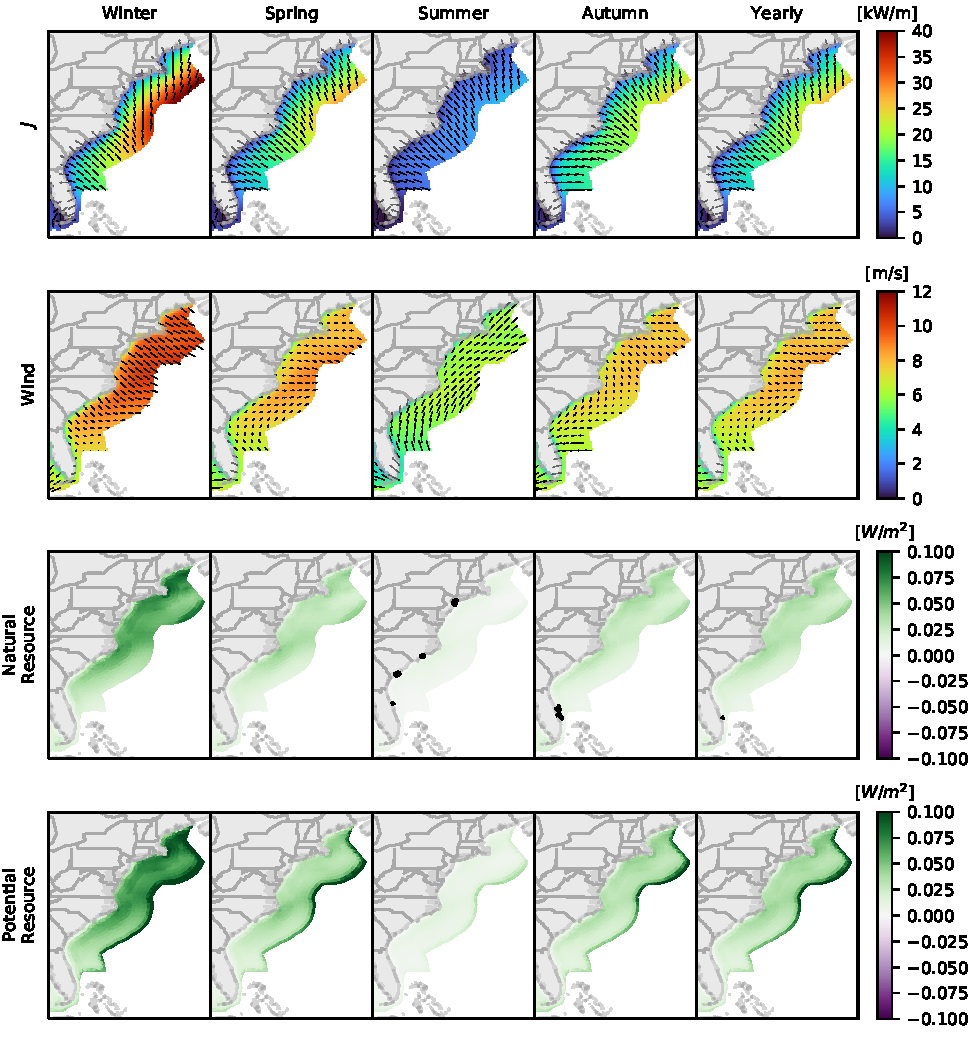
\includegraphics[width=\textwidth]{../fig/at_spatial_seasonal_mag_4.pdf}
%   \caption{Same as \ref{fig:maps-at} for East Coast.}
%   \label{fig:maps-at}
% \end{figure}

\begin{figure}[ht]
  \centering
  \includegraphics[width=\textwidth]{../fig/AnnualCycle01.pdf}
  \caption[Wave resource annual cycle.]{The annual cycle of the total wave energy resource for several regions, relative to the regional mean.}
  \label{fig:annual-cycle}
\end{figure}


%\begin{figure}[ht]
%  \centering
%  \includegraphics[width=\textwidth]{../fig/AnnualVar01.wc.pdf}
%  \caption[West Coast resource variability.]{Annual and inter-annual variability of the West Coast resource. The thick solid line indicates the mean, and the orange lines and boxes indicate the median and quartiles, respectively. The whiskers extend to the last point within 1.5x of the inter-quartile range, and points beyond this are plotted as open-circles.}
%  \label{fig:wc-variability}
%\end{figure}

\begin{figure}[ht]
  \centering
  \includegraphics[width=\linewidth]{../fig/TotalResource_Freq02.pdf}
  \caption[Distribution of wave energy vs. wave-period.]{Distribution of wave resource by wave period for each region. Each line represents a spatial average over the entire regional domain. Thick lines indicate the remote resource only, thin lines indicate the sum of the potential and remote resource. Colors are used for each region. Each curve is normalized by its total energy (i.e., the integral of each curve is 1).}
  \label{fig:remote-freq}
\end{figure}

%%% Local Variables:
%%% TeX-master: "wave_res"
%%% End:

\section{Discussion} \label{sec:discussion}

Including the natural or potential local resource in estimates of total theoretical wave energy assessments -- as we propose here -- is a fundamental change in methodology. There are several practical questions about how this energy can be harnessed on both large and small scales. 
Most importantly, we note that the ``potential local'' resource only becomes available when large-scale wave energy extraction becomes economically feasible at great distance from shore. Even the ``natural local'' resource doesn't become a significant component of a wave energy projects resource until the size of the project is greater than several thousand square kilometers. As an example, consider fetch limited wave growth under a constant 10 m/s wind in deep water. Following \citet{donelan1980similarity} it will require 50 km of fetch for waves to have a modest wave flux of 1.5 kW/m. 
% \note{Need to check on these numbers.}\textcolor{green}{We can reference the fetch limited wave growth formulae here if that is what you had in mind.} \note{That's exactly what I'm looking for here! Thanks! Can you add that?} Yes

There is also work to be done in understanding how much of the local resource overlaps with the offshore wind resource (i.e., does extracting wave energy -- so that the wave surface is flatter -- reduce or increase the offshore wind resource?). Along these lines, and especially in locations where the seasonality of OSW compliments the wave resource (e.g., as noted in section \ref{sec:results:wc-dist}), it is intriguing to consider the development of projects designed to harness both wave and OSW energy. The methodology proposed here is well suited to evaluate this opportunity, but that is left for future work.

There is also the question of what kinds of devices will efficiently harness this relatively high-frequency energy. 
Will devices of the future be sufficiently broad-banded to extract the local resource and remote resource equally efficiently? 
What technological changes are required to make that happen? There is use for this energy in niche blue economy markets, or if energy storage technologies (e.g., liquid renewable fuels) become sufficiently inexpensive. If so, will the WEC technologies be economically competitive? 

Harnessing the extra energy in the {\em potential} local resource provides even greater challenges. In particular, tapping into this piece of the wave resource will require extracting large fractions of the remote resource very far from shore, so that their is sufficient fetch for waves to grow and be harnessed by WEC arrays inshore.  

Though these issues exist, we still propose that including the local resource in the total is important for several reasons. First and foremost, it is a real part of the total energy that is contained in the resource, and available for conversion to electricity. Therefore, it falls squarely in the IEC definition of ``theoretical resource''. Second, including it resolves outstanding questions associated with earlier resource assessments (i.e., ``how much energy is available inshore of a chosen boundary?''). This question is especially addressed/resolved by the {\em potential} local resource. And third, including it broadens our understanding of what wave energy is. That is, there is a significant amount of energy at relatively high frequency that could be useful for PBE applications that require relatively small amounts of power. Furthermore, the methodology proposed here -- which has been applied at a regional scale -- can also be applied at the project scale (e.g., down to a single device represented by a small box).
This accuracy at all scales makes it ideally suited for broader adoption by the international community, which will in turn make the assessment of market opportunities more comparable and transparent.

Currently, the IEC Wave Resource Assessment technical specification (TS) focuses on quantifying resource parameters that are important to characterizing the resource across different spatial scales (i.e., three "classes" of resource assessment), but it provides little guidance on how to sum the theoretical resource for a region or site of interest. This is because this technical specification is focused primarily on characterizing the resource for feasibility studies (class 1 and 2) and quantifying the resource for designing projects where technologies are known (class 3). At the feasibility level, omni-directional wave power serves as a useful metric for quantifying the opportunity for wave energy development. When conducting array design, the TS states that ``the effects of the WEC array on wave propagation should be included in the numerical model. Any modifications made to the numerical model to account for the effects of a WEC array shall be documented and justified.'' This is important guidance that effectively accounts for wave directionality, but it is not practical or feasible when performing large-scale theoretical resource assessments for arbitrary devices. Instead, the approach used here skips the complexity of simulating many (thousands to millions or more?) of individual WECs extracting energy, and instead treats the line as a `perfect' array that extracts all of the incoming energy. By using a line-integral (dot-product), we are accounting for the directionality of waves (i.e., the `shadowing effect' of arrays) that is called for in the standards. Thus, the line-integral approach effectively accounting for the `shadowing effect' that is required by the IEC TS, and therefore this approach is consistent with it.


In the intro we state that this work is motivated by a desire to bring clarity to regional RA, but in the end we find that the -- because the methods developer here are scalable -- they are potentially of value to site-focused assessments as a means to estimating total theoretically-available power over a specified project/site area.

The methodology described in section \ref{sec:method} can also be used for site-assessments to estimate the total power available within the project area. However, when the project size is less than a few thousand sq. km. the local (both natural and potential) are unlikely to change the result by more than a few percent. Thus, for site-assessment, neglecting the local resource term (i.e., avoiding the additional work of calculating it) is accurate to within a few percent points.
For cases where storing the source terms, $S$, from the model is straightforward, and if a user does want to use the method at the project-scale, the approach is identical to that described here. The one-way line-integral should be performed along the boundaries where the project has rights to the incoming wave energy, and the `local resource' is estimated using \ref{eqn:RL} over the area of the project site. 

\subsection{The potential for wave energy in the U.S.}

The U.S. has vast wave energy resources. The West Coast is typically viewed as the premier U.S. market because the resource magnitude and intensity are both high, and the West Coast energy market is large. The west coast theoretical resource (420~TWh/yr) is equal to about 45\% of electricity consumption by the three coastal states there (CA, OR, WA 2018 total: 943 TWh/yr), which indicates that their is sufficient resource to play a sizable role in the region's energy profile \citep{energyinformationadministrationStateEnergyConsumption2020}.  
The fact that the remote wave energy resource here complements the offshore wind resource in several locations, suggests that OSW-wave hybrid projects might have higher annual capacity factors than projects involving one of these technologies alone. The PacWave test site, offshore of central Oregon, has been created to be the first U.S. "grid-connected full-scale test facility", which will provide the opportunity to develop and demonstrate technologies in this world-class ``fully energetic'' resource where winter storms can deliver wave amplitudes greater than 8 meters \citep[e.g.][]{allan_climate_2006}.

Though Alaska has a larger total resource than the West Coast, the majority of this is `stranded'. That is, it is located very far from large populations where markets are large enough to attract projects bigger than a few MW. Still, the wave resource along Alaska's Aleutian chain is sizable, and raises the possibility of the export of Alaska's wave resource if and when large-scale energy storage technologies become sufficiently economical (e.g., liquid fuel storage, batteries, etc.). Could a breakthrough of this kind reignite Alaska's energy-export economy, this time for Alaska's vast renewable energy resources? In the shorter-term, the villages along Alaska's coastline -- where energy prices are very high -- represent an opportunity to demonstrate commercial viability before scaling the technology up \cite{alaskaenergyauthority2019PowerCost2020}. Or this energy could be used in-place, to charge batteries on vessels or scientific instruments during long transits or exploration. 

Hawaii possesses a relatively large resource (~430 TWh/yr total, 120 TWh/yr inner-shelf) considering the State's population and electricity consumption (26 TWh/yr), and is an especially attractive early market for wave energy because of the high-energy prices there. 
Wave energy may be particularly valued in Hawaii where space is limited for land-based renewable alternatives; the tourist economy there may especially value WECs with limited surface expression. Together, these factors make Hawaii a likely early-market for wave energy technology. The Navy's Wave Energy Test Site on the north shore of Oahu, is supporting the development and demonstration of technologies for meeting the potential demand \citep{crossEarlyResearchEfforts2015}.

The East Coast and Gulf of Mexico wave resources are modest in comparison to the above regions. Still, it is too early to neglect the potential for wave energy in these regions. As wave technologies continues to mature and if the cost of the technology is low enough, sites and regions previously considered uneconomical may prove to be attractive, especially in markets where energy prices are already high and alternate renewable sources are limited or constrained. Small grids such as those in Puerto Rico, the U.S. Virgin Islands, and in remote Alaska are struggling to identify affordable and reliable local sources of power. Wave energy could help to fill periods of time when other sources of energy are unavailable (renewable or not), thereby increasing the resiliency of the grid-system.

\subsection{Predictability of wave energy}
One of the main advantages of wave energy is the idea that it is much more predictable than most other renewable energies. On daily to weekly timescales, wave can be predicted by wave propagation models driven be realtime storm data from ocean basins. On inter-annual timescales, several works have noted a correlation with ENSO fluxuations. Figure \ref{fig:wc-nino} compares the West Coast remote wave resource anomaly (the deviation from the annual mean) to the Oceanic Nino Index (ONI) lagged by 2 months. \cite{nationaloceanicandatmosphericadministrationOceanicNinoIndex2020}.
Here we see a strong correlation between the highest values of the west coast resource and high values of ONI. The fact that the wave resource lags the ONI suggests that the ONI can be used to predict peaks in wave energy. This correlation is likely to be causal because ENSO events are correlated with larger storms in the S. Pacific, which is a major source of wave energy on the U.S. West Coast \citep{andersonClimateIndexOptimized2018, yangCharacteristicsVariabilityNearshore2020, ruggieroNationalAssessmentShoreline2013}.
On shorter timescales, modern improvements in wave modeling have made significant advances in the accuracy of wave prediction \citep{cavaleriWaveModellingCoastal2018}. Applications of artificial intelligence have also shown promise for accurate prediction of wave height and wave power \citep[e.g.][]{cornejo-bueno_significant_2016}. This predictability, and the degree to which wave energy compliments other types of renewable energy in specific locations, may become increasingly valuable as electrical grids are powered increasingly by variable renewables \cite{parkinsonIntegratingOceanWave2015}.

\begin{figure}[ht]
  \centering
  \includegraphics[width=\textwidth]{../fig/ENSO-Comparison.wc.pdf}
  \caption{West Coast wave energy flux anomaly vs. oceanic nino index. The wave energy flux anomaly (annual cycle removed) is averaged along the EEZ boundary, has had a 5-month running average applied, and lags the ONI signal by 2-months.}
  \label{fig:wc-nino}
\end{figure}


\section{Conclusion} \label{sec:conclusion}

We propose a methodology for theoretical wave resource assessment that resolves several outstanding issues with earlier approaches. In particular, this work accounts for wave directionality in order to reduce `double counting', and also includes the energy added to the wave field by local winds. This provides a consistent methodology for accounting for wave energy at national/regional scales. So that policy makers can have a clear understanding of wave energy potential. As other nations/regions adopt the methodology, we will have an apples-to-apples comparison of opportunity, which can inform decision making and investment.

We then apply this methodology to the U.S. EEZ (except for the portion of the EEZ associated with U.S. Pacific Islands Territories), and find that the total U.S. wave energy resource is greater than 3,300 TWh/yr.
This is an increase of ~25\% compared to earlier DOE wave resource assessments, and is due to the combination of extending the resource area to the edge of the EEZ and incorporating the local resource. The `inner shelf' resource also increases from a total of ~1600 TWh/yr in EPRI 2011 to 1800 TWh/yr here, but the majority of this increase can be attributed to Alaska \textcolor{blue}{Most of the increase is in AK. Why?! ... The 'inner shelf' remote resource is > than the EEZ remote resource. Is this just because the contour is longer? Is it worth discussing this nuance in RESULTS or DISCUSSION?}

A detailed assessment of the ``technical resource potential'', which accounts for the efficiency and array design of existing technologies is left for future work. Furthermore, an assessment of the ``practical resource'' is a greater challenge because it requires accounting for regional permitting details, ocean-planning designations, and competing uses by other ocean stakeholders.

We encourage the IEC wave resource assessment team to consider adopting pieces of this methodology in the ``reconaissance'' level assessments in order to promote the adoption of consistent regional resource assessments methods. Furthermore, the methods proposed here could also be of use to project developers in identifying the maximum resource potential of a project site. \textcolor{blue}{Need to think about how to say this more tactfully.}


%%% Local Variables:
%%% TeX-master: "wave_res"
%%% End:


\section*{Acknowledgements}
This work was authored by the National Renewable Energy Laboratory, operated by Alliance for Sustainable Energy, LLC, and by Pacific Northwest National Laboratory, operated by Battelle for the U.S. Department of Energy (DOE) under Contract Nos. DE-AC36-08GO28308 and DE-AC05-76RL01830 (respectively). Funding was provided by the Office of Energy Efficiency and Renewable Energy Water Power Technologies Office. All model simulations were performed using resources available through Research Computing at Pacific Northwest National Laboratory. The views expressed in the article do not necessarily represent the views of the DOE or the U.S. Government. The U.S. Government retains and the publisher, by accepting the article for publication, acknowledges that the U.S. Government retains a nonexclusive, paid-up, irrevocable, worldwide license to publish or reproduce the published form of this work, or allow others to do so, for U.S. Government purposes. 

The authors are also grateful to many colleagues for innumerable discussions and reviews that helped to improve the method, results, and quality of this manuscript. George Hagerman and George Scott, both provided data and lengthy discussions that helped to improve the accuracy of the results and clarify the method. H. Tuba \"{O}zkan-Haller, Mark Hemer, and Jim Thomson provided their expert perspective that was especially valuable in defining the local resource. We thank Alejandro Moreno, Hoyt Battey, Steve DeWitt, Michael Lawson, and Bob Thresher for supporting the work and encouraging a comprehensive approach. Kathleen Morton, Aidan Bharath, John Frenzl (Figure \ref{fig:diagram:west-eez}), and Billy Roberts (Figure \ref{fig:map-total}) helped to create the graphics; this report wouldn't be the same without them. We also are sincerely grateful to Becki Meadows and Caroline Draxl for multiple insightful reviews and detailed editing of several versions of this manuscript.

\appendix
\setcounter{figure}{0}
\section{On the details of estimating the remote resource} \label{appendix:one-way-method}

\subsection{The importance of accounting for wave directionality}
\label{appendix:directionality}

As the US National Academy of Sciences review points out, estimates of the remote resource $R_R$ must account for wave directionality in order to avoid double-counting of the wave resource \citep{nationalresearchcouncilEvaluationDepartmentEnergy2013}. For example, when a wave with energy density of $1 \unit{kW/m}$ crosses a $1 \unit{km}$ integration contour segment with its wave crests parallel to the segment, the total power is 1MW (upper row of Figure \ref{fig:directionality}). Likewise, when that same 1-km wide wave crosses a contour-segment with its wave crests at an angle to the integration contour, the total energy contained in the wave is still only 1 MW. The directionality coefficient corrects for the fact that the length of the contour segment is longer to capture the whole 1-km wave at an angle (3 km in lower row of Figure \ref{fig:directionality}, where $\Delta\theta = \theta_n - \theta = 70.5^{\circ}$). In the `unit circle' method described in the EPRI 2011 resource assessment \citep{EPRIwaveresource2011}, $\delta$ is taken to be $1$ in all cases (directionality is neglected), which for the wave depicted in the lower row of Figure \ref{fig:directionality} gives an estimate of 3 MW crossing the contour. This is clearly incorrect since the 1-km wide wave only contains 1 MW of power, and demonstrates the importance of accounting for directionality.

\begin{figure}[ht]
    \centering
    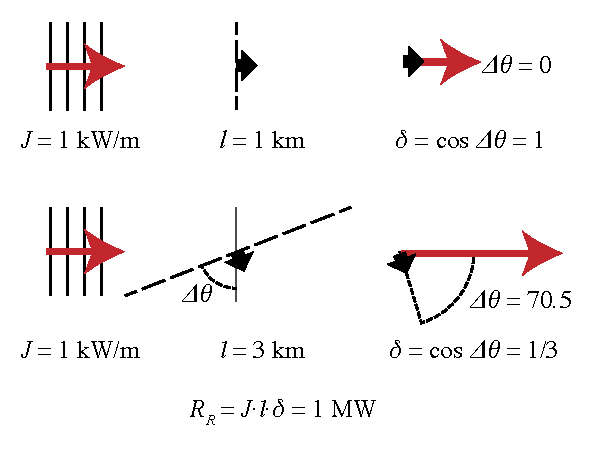
\includegraphics[width=0.6 \linewidth]{../../diagram/Dot-Product_Schematic}
    \caption{A diagram depicting the importance of accounting for wave directionality. The upper sequence depicts a scenario where wave crests are parallel to the integration contour ($\delta = 1$), and the lower row is a scenario where wave crests are oblique to the contour ($\delta = 1/3$). The arrows represent the direction of wave travel.}
    \label{fig:directionality}
\end{figure}

One of the main reasons there has been confusion about this topic is due to the fact that many types of WECs are agnostic to the direction that wave energy arrives from (Figure \ref{fig:omni-dir}A, and EPRI 2011 Figure 2-13). That is, all other things being equal (wave height, period, etc.), these `omnidirectional WECs' generate the same amount of power regardless of the direction that wave energy arrives from. For a single WEC of this type, it is possible to obtain an estimate of power output by simply multiplying the device's capture-width by the omnidirectional wave power. However, when many of these devices are arranged in an array where their spacing is close enough to capture all of the incident energy, then they begin to shadow one-another in a way that depends on wave direction and array-layout (i.e., in a similar manner to how wind turbine wakes reduce the performance of down-wind turbines).

Accurately modeling arrays of devices is technically challenging at regional scales, but the point here is that directionality matters for WEC arrays, and these arrays cannot generate more energy than exists in the waves. For the purposes of theoretical wave resource assessment then — instead of attempting to model arrays of devices that extract all of the energy in the wave-field — we simply draw an integration contour and assume that we can extract all of the energy that crosses it using \eqref{eqn:RR}. In other words, omnidirectional wave power is useful for quantifying the intensity of wave energy at a point and in spatial maps, but it cannot be used as a replacement for wave energy flux when performing line-integrals of the wave resource.

\begin{figure}[ht]
    \centering
    \fbox{\includegraphics[width=0.3\linewidth]{../../diagram/omni-dir01}}
    \fbox{\includegraphics[width=0.3\linewidth]{../../diagram/omni-dir02}}
    \fbox{\includegraphics[width=0.3\linewidth]{../../diagram/omni-dir03}}
    \caption{A) A ``point absorber'' type omni-directional WEC is denoted as a black circle. B) Though a single ``point absorber'' does not care about wave-direction, an array of such devices does because individual devices shadow one-another depending on wave direction. C) Shadowing is indicated explicitly in this case where the array is a line of ``point absorbers' spaced close enough to capture all incoming energy.\textcolor{blue}{These figures are place-holders for now. }}
    \label{fig:omni-dir}
\end{figure}

\subsection{A detailed discussion of the `one-way' approach to estimating the remote resource}

The one-way approach to estimating $R_R$ deserves some explanation because it deviates from the traditional definition of a line-integral.

A key piece of this discussion rests on the fact that \eqref{eqn:RR} is typically computed from wave models that do not simulate the removal of the wave energy when it encounters the integration contour of interest (e.g., $\leez$). This means that, in the long time-average used in \eqref{eqn:RR}, wave energy that crosses a contour at one location may also be crossing the contour at another location at another time in the average, which can lead to over- or under-counting that wave. Without revising the model to extract the energy at the contour there is no way to know for sure whether there are waves that are being under- or over-counted in the estimate of $R_R$. Revising the model to extract wave energy that encounters the boundary, and account for it according to \eqref{eqn:RR}, is no simple task.

In a traditional line-integral, the directionality coefficient is simply:
\begin{align}
    \delta_{*} = \cos(\Delta \theta)
    \label{eqn:trad-def}
\end{align}
The primary problem with this definition for the purposes of wave resource assessment is that waves that propagate away from the shoreline of interest ($|\Delta \theta | > 90$) are subtracted from the resource total. To avoid this we utilize the `one-way' condition for summing wave energy:
\begin{align}
    \delta = 
    \begin{cases}
     \delta_* & \mathrm{for\ }|\Delta \theta|<90^\circ \\
    0 & \mathrm{otherwise}.
    \end{cases}
    \label{eqn:1way-def}
\end{align}

The primary draw-back to the one-way condition is that if wave energy criss-crosses back-and-forth across the integration contour, then it is added to the total each time it crosses the contour (rather than being counted, correctly, exactly once). However, since waves do not typically swerve back and forth (i.e., across a straight line), this should only be an issue when the integration contour zig-zags or otherwise has segments that a straight-travelling wave would cross multiple times (e.g., where the contour folds, or when islands are spaced such that there are several independent contours nearby one another).

\begin{figure}[ht]
    \centering
    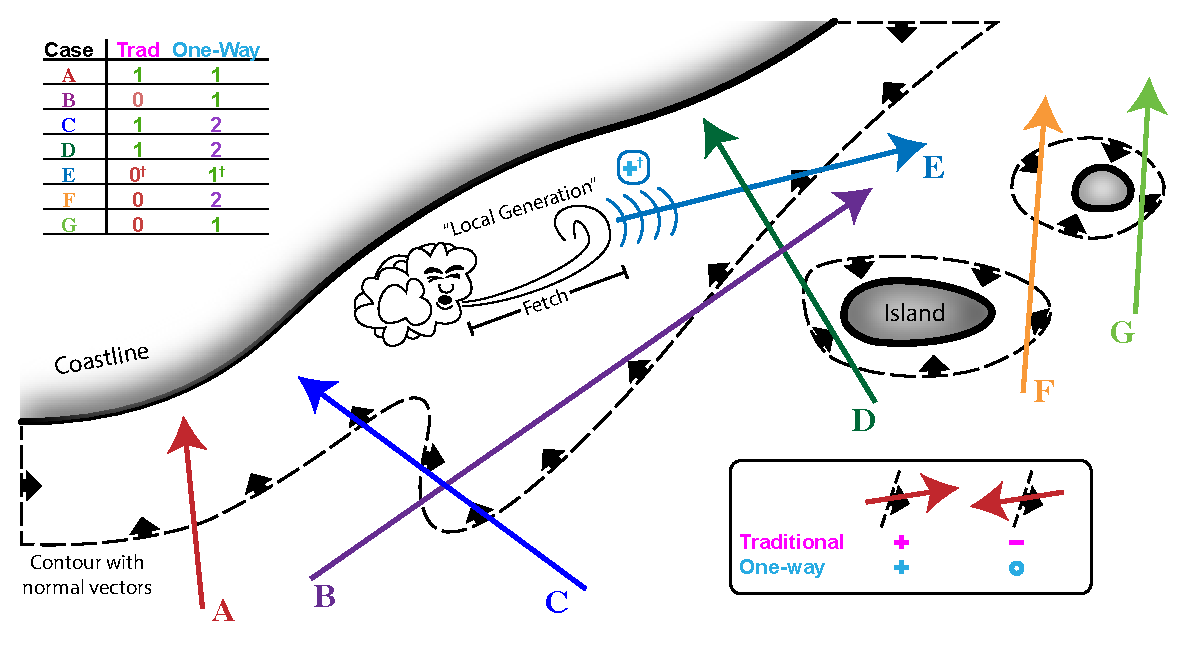
\includegraphics[width=\linewidth]{../../diagram/Schematic03.pdf}
    \caption{A diagram depicting different cases of waves (color arrows) crossing an arbitrary integration contour (black dashed line). Black arrows along the contour indicate the contour-normal direction. The lower-right legend indicates whether energy is added to (+), subtracted from (-), or neglected ($\circ$) in the total where waves cross the contour. The upper-left legend indicates the `count' for each wave for the two methods. The `blowing cloud' image indicates the generation of `local waves' over the region bounded by the integration contour.}
    \label{fig:one-way-diagram}
\end{figure}

Figure \ref{fig:one-way-diagram} provides a schematic of several cases of wave energy (color arrows) propagating across an arbitrary integration contour (black dashed line). A traditional dot-product adds the energy when a wave crosses into the contour, and subtracts that energy when it passes outwards across the contour (pink row in lower right legend). The `one-way dot product' adds the energy wherever it crosses into the domain, and neglects it when it crosses outward (cyan in lower-right legend).

The arrows depict several different cases of wave energy crossing the contour. Arrow `A' indicates the most-common case of a wave crossing into the contour from offshore exactly once. Arrow `B' is a case where a wave propagates into and out-of the integration boundary. Arrow `C' is the case where a wave crosses a zig-zagging countour several times. Arrow `D' is the case of a wave propagating through an island's contour before entering the mainland contour. Arrow E is the case of a wave that is generated within the domain (i.e., locally). Arrows F and G are cases involving waves passing by islands.

The upper-left legend indicates the number of times each wave is counted using the `traditional' and the `one-way' dot-product. The correct answer is that each wave should be counted exactly once for all cases. The first thing to note, then, is that neither method gets it right in all cases. The traditional method ignores several waves, while the one-way method double-counts several. Also note here that we have included the `local resource' for arrow E (marked by $\dagger$).

The one-way method is correct for several cases that would seem to be relatively common such as arrows B, E, and G, while the traditional method neglects them completely. The one-way method is only incorrect when a wave crosses a zig-zagging section of the contour (C), or when it crosses adjacent distinct contours (D, G). Therefore, as long as the integration contours are relatively straight and there are not multiple contours in close proximity, the one-way method should produce reasonably accurate results. 
The relevant length scale for defining `relatively straight' and `close proximity' is the scale over which wave energy propagates, which obviously spans ocean basins. However, it seems reasonable to assume for the EEZ boundaries we explore here, that zig-zagging is minimal and the individual boundaries are sufficiently far-apart to minimize double-counting. On the other hand, the use of the traditional dot-product is likely to result in significant under-estimation of the resource because cases E and G are very likely to occur in many scenarios. Therefore, it is straightforward to conclude that the exact answer lies somewhere between the one-way and traditional method, but in most cases is probably much closer to one-way.

We did calculate the remote resource ($R_{R*}$) using the traditional dot-product by replacing $\delta$ with $\delta_*$ in \eqref{eqn:RR}. These results show that $R_{R*}$ is smaller than $R_R$ by 20 to 100\% (Table \ref{tab:RR*}). This can be explained for most regions by assuming that 40-60\% of the locally generated waves propagate offshore. In Hawaii, where that approach does not work, the answer is clearly that a large fraction of the wave energy simply passes into and back-out-of the domain, and is therefore erroneously ignored by the traditional dot-product.

\begin{table}[ht]
  \centering
  \begin{tabular}{cccc}
  \hline
  Region & $R_R$ & $R_{R*}$ & $R_{L}$ \\
  \hline
  Alaska & 1040 & 430 & 990 \\
  West Coast & 420 & 360 & 90 \\
  Hawaii & 370 & 80 & 10 \\
  East Coast & 110 & 0 & 180 \\
  Gulf of Mexico & 13 & -2 & 56 \\
  P.R. \& U.S.V.I. & 6 & 4 & 11 \\
  \hline
  \end{tabular}
  \label{tab:RR*}
  \caption{A comparison of remote resource computed using the one-way method ($R_R$) to a traditional dot-product ($R_{R*}$), and the local resource ($R_{L}$). All values in TWh/yr.}
\end{table}

The only way to avoid this error completely is to extract wave energy in the model simulation at the integration contour of interest -- and account for it according to \eqref{eqn:RR} -- so that it does not propagate to a different point on the contour where it could be mis-counted. This approach, however, is technically challenging and reduces the flexibility of data analysis because a new simulation must be run for each contour of interest.

\subsection{On the proximity of regional domains}

The issue of `double counting' arises again with this method, as discussed above, when two or more nation's EEZs are in close proximity to one another, but not quite touching. The gulf of Mexico provides an example of this: Mexico's EEZ pushes up against the U.S. EEZ. Clearly the majority of wave energy propogating north across the U.S.'s southern EEZ boundary originated within Mexico's EEZ, and therefore is technically Mexico's resource. It could be harvested by WEC farms and never make it to the U.S. In this case, the U.S.'s remote resource in the gulf is less than 20\% of its local resource, so it does not play a major role in the total there, nor does it contribute significantly to the nation's resource. Thus the remote resource along lines that separate neighboring countries' EEZs should not be included in the assessment. 

% \begin{figure}
%     \centering
%     \includegraphics[width=0.7\textwidth]{../../fig/at_EEZ_resourcePlot}
%     \caption{The U.S. EEZ along the east and gulf coasts (burgandy). The thick solid line separates the EEZ from the open ocean (where $R_R$ is calculated), and dashed lines are borders with other nation's EEZs.}
%     \label{fig:at-EEZ}
% \end{figure}


%%% Local Variables:
%%% TeX-master: "wave_res"
%%% End:

\setcounter{figure}{0}
\section{Comparing wave flux divergence to source term area integral}\label{appendix:flux-vs-area}

To the authors knowledge the source term method for computing the local wave resource is being introduced in this work for the first time. Since the source term method cannot be validated directly, it will be compared against the results obtained from the energy flux method under idealized conditions. The local resource using the energy flux method under idealized conditions is computed by subtracting the wave energy flux exiting the domain from that entering the domain using Equation~\eqref{eqn:RR}. In the absence of sources and sinks of energy other than wind input, dissipation due to whitecapping, and quadruple interactions, the difference between the incoming and outgoing energy flux reveals the local resource.

WW3 is implemented in an idealized model over a bathymetry with a constant depth of 4 km covering a region that is 240$^{\circ}$ in the zonal direction and 60$^{\circ}$ in the meridional direction as shown in Figure~\ref{fig:idealizedDomain}a. Deep water was selected to remove the effects of energy convergence or divergence by refraction, and shallow water effects such as depth-induced wave breaking and bottom friction. We consider a hypothetical EEZ as a proxy for a region of interest. Energy flux is computed at 200 nautical miles from the eastern end of the domain, which we approximate in the model as 3$^{\circ}$20’ from the eastern boundary given the model domain has been centered at the Equator. This hypothetical EEZ covers 20$^{\circ}$ in the meridional direction as shown in Figure~\ref{fig:idealizedDomain}a. The area of this region is 818,000 km$^{2}$, which is comparable in size to the US West Coast EEZ (825,550 km$^{2}$). In the meridional direction the model spatial resolution is a constant 1$^{\circ}$ (111.12 km), while in the zonal direction the spatial resolution is reduced from 1$^{\circ}$ (111.12 km at the Equator) to 4’ (7.4 km) close to the EEZ (see Figure~\ref{fig:idealizedDomain}b) to be consistent with the models used in the hindcast.
 
\begin{figure}[ht]
  \includegraphics[width=4.5in]{./fig/appendixB_Figure1.png}
  \caption{a) Idealized model grid with the analysis zone identified with a red box. Continents are added for visualizing the scale of the model only, the model domain is a basin with constant depth. b) Zonal resolution of the model grid.}
  \label{fig:idealizedDomain}
\end{figure}

For all the idealized simulations, a stationary 7.0 m/s westerly wind is applied over the entire domain. The wind speed is based on the yearly averaged wind speed measured at NDBC stations 46005 and 46002 offshore the U.S. West Coast (\url{https://www.ndbc.noaa.gov/}), which are 7.3 and 7.0 m/s, respectively. The model domain was selected to be long enough such that the waves achieve energy equilibrium (i.e., constant wave height and period) west of the analysis zone. The model is executed for three months, where the results from the first two months are discarded to ensure steady state. The two methods of computing the local resource, energy flux and source term, are compared by analyzing two different scenarios of the idealized model. For both scenarios, the model is forced by a constant westerly wind west of the EEZ but only one of them has local wind forcing east of the EEZ. Wave energy flux collected at the end of the simulation period along the Equator is shown in Figure~\ref{fig:idealizedOWP}. The results are consistent west of the EEZ where the wind is active in both cases. The remote resource is computed along this line and is very similar for both scenarios as shown in Table~\ref{table:idealizedResource}. There is a decrease of wave power just westward of the EEZ (where the wind stops acting), which is attributed to the northern and southern model open boundaries having upstream effects on the wave field.

\begin{figure}[ht]
  \centering
  \includegraphics[width=3in]{./fig/appendixB_Figure2.png}
  \caption{Wave energy flux across the middle of the domain with and without local wind forcing.}
  \label{fig:idealizedOWP}
\end{figure}

In the case of no local wind the wave power starts decreasing quickly eastward of the EEZ. This is because of the swell dissipation component of $S_{in}$ source term \citep{ardhuinObservationSwellDissipation2009}. The total dissipation rate decreases eastward due to the propagation of the swell in this direction. The local resource for such a scenario is negative. It is worth noting that the contribution of $S_{ds}$ to the total balance is zero because there is no active wave growth that would be balanced by whitecapping. The local wave energy resource from both approaches yield similar results as shown in Table~\ref{table:idealizedResource}. In this example the loss of wave energy amounts to 37\% of the remote resource. 

On the other hand, when the waves have reached a stead state (known as a fully developed sea), the local wave resource is, by definition, zero. Computing the local resource from both approaches yield results very close to zero as well (Table~\ref{table:idealizedResource}). For this condition the wave energy flux is constant with longitude (as observed from Figure~\ref{fig:idealizedOWP}) and, based on our definition, computing the energy flux across different meridians and subtracting them will result in zero local resource. In this case swell dissipation is countered by wind wave growth at high frequencies which is then transferred to the lower frequencies via the non-linear interactions.

\begin{table}[ht]
  \centering
  \begin{tabular}{cccc}
    \hline
    Local Wind & Remote Resource & Local Resource: Energy Flux & Local Resource: Source Terms \\
    \hline
    No  & 12.94 & -5.44 & -5.49 \\
    Yes & 13.42 & -0.02 &  0.15 \\
\hline
  \end{tabular}
  \caption{Wave energy resource for idealized basin in GW}
  \label{table:idealizedResource}
\end{table}

Both approaches produce very similar results given that the waves have an eastward travel direction, thus avoiding the shortcomings of the energy flux method discussed in Section~\ref{sec:method}. Therefore, the source term method is suitable to estimate the local resource.

\setcounter{figure}{0}
\section{Stations for model-data comparison}\label{appendix:validation}

\begin{sidewaysfigure}
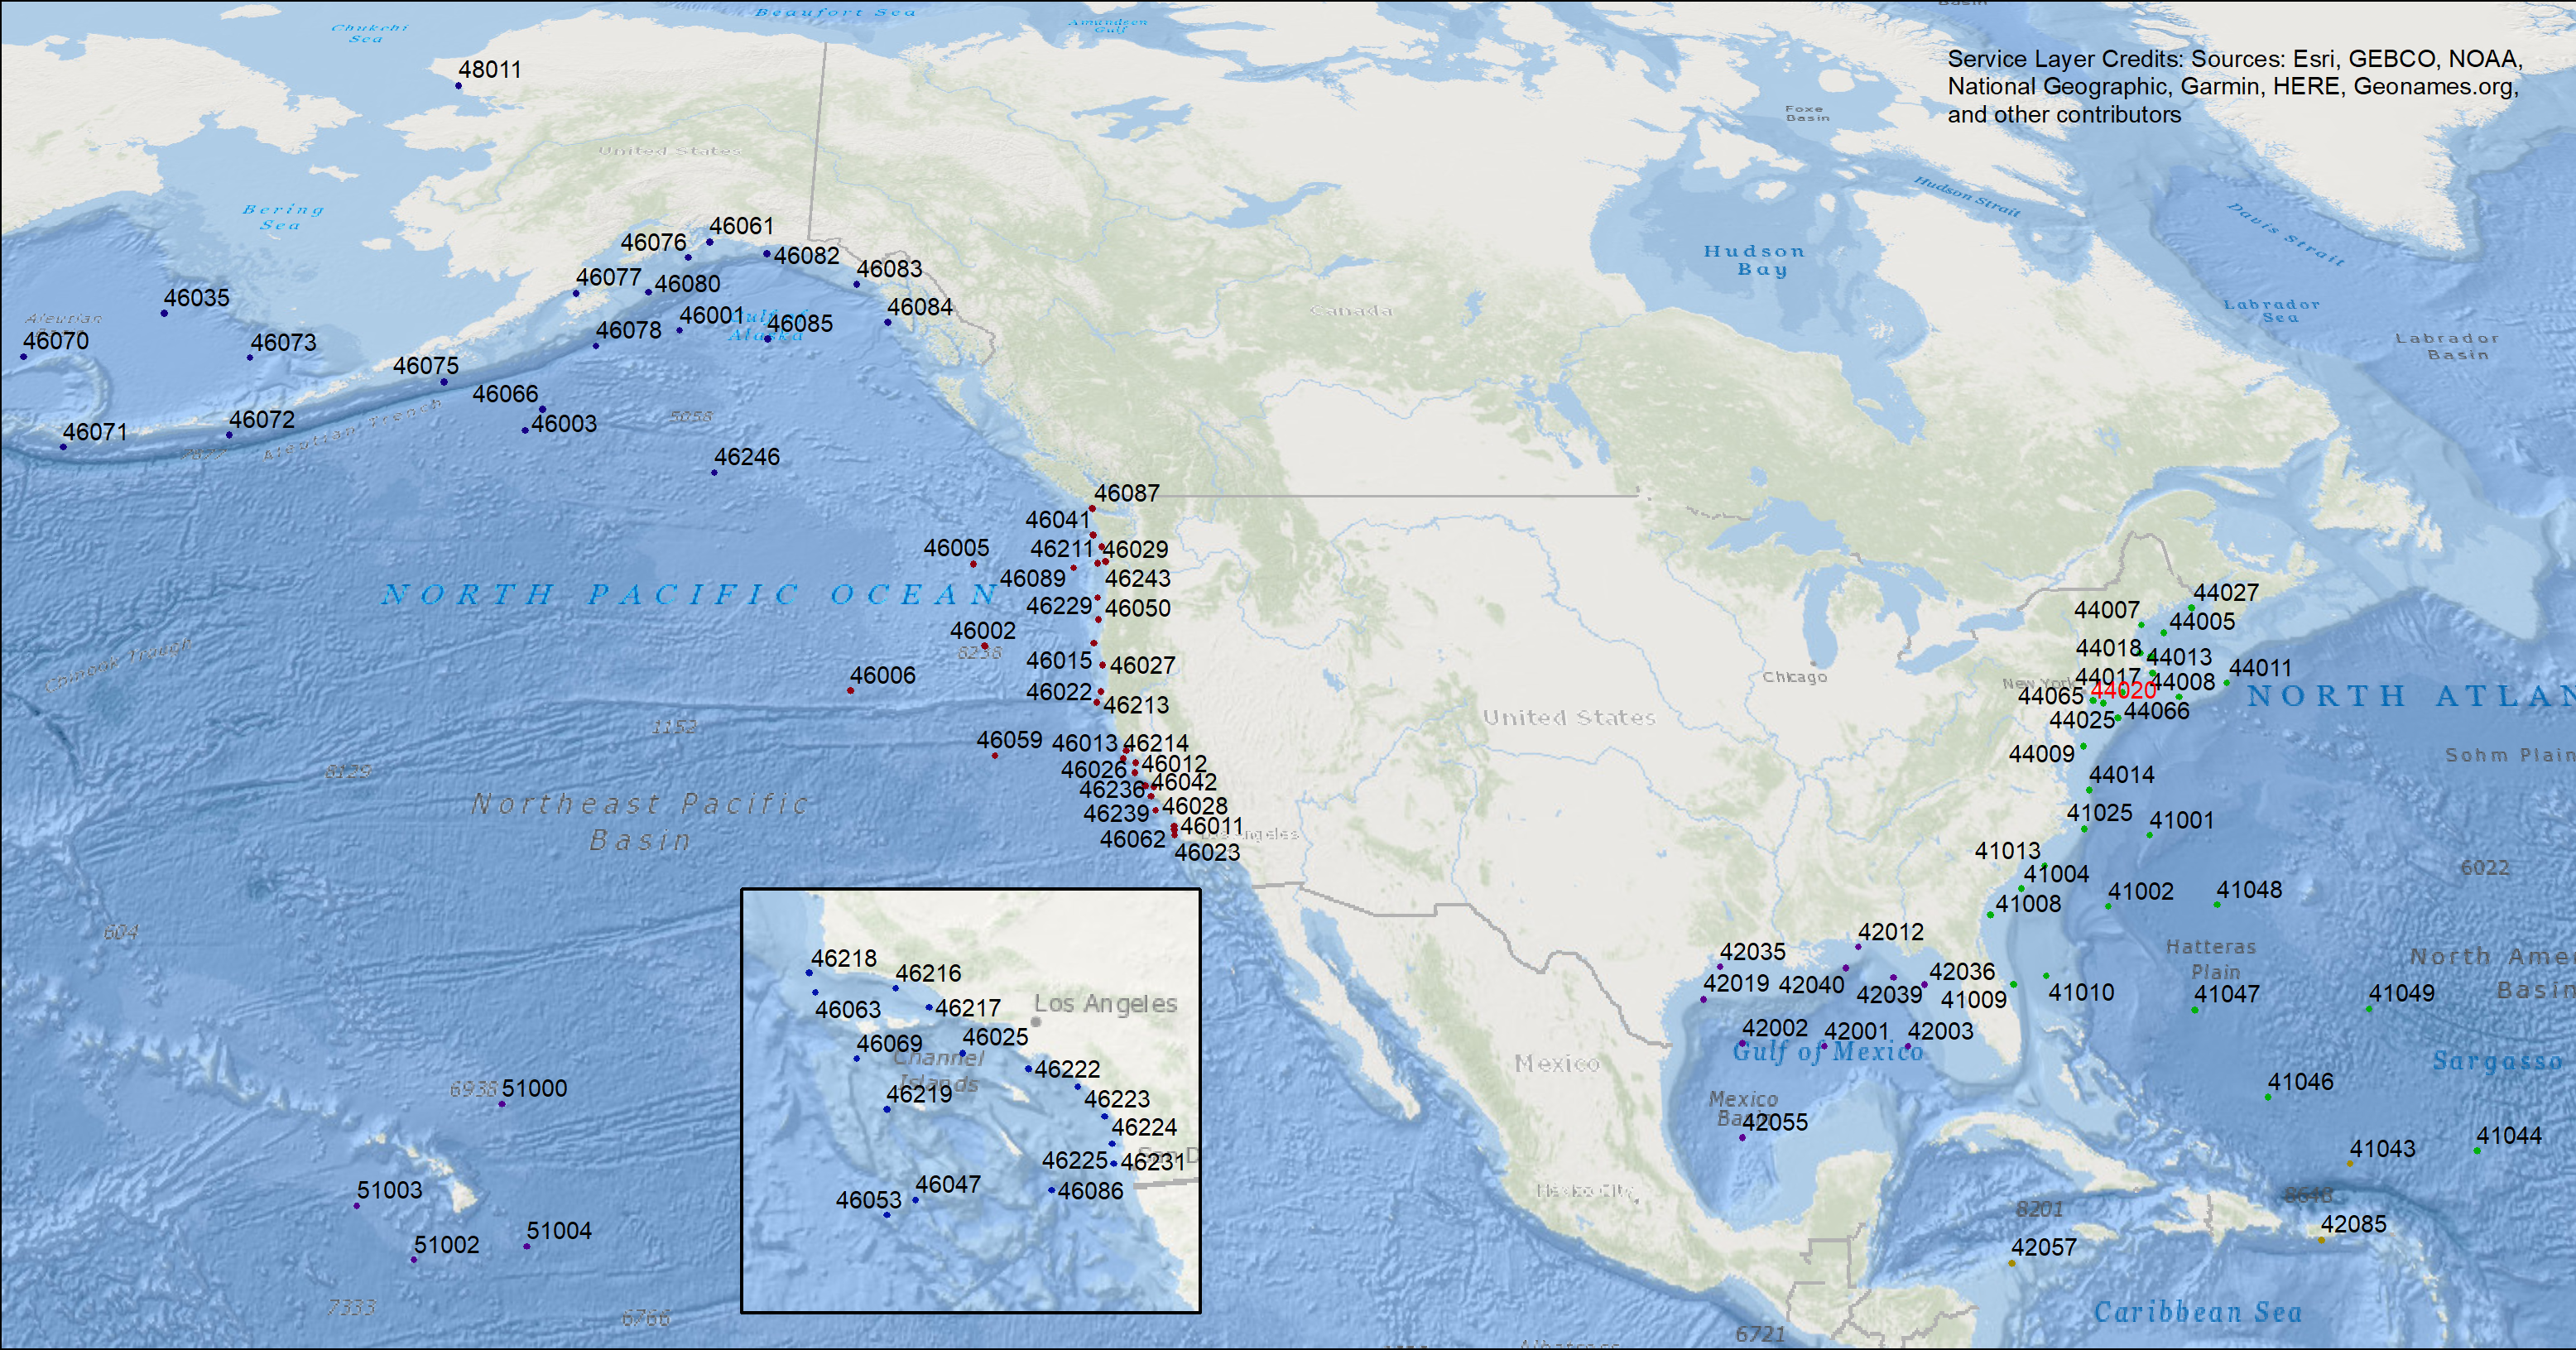
\includegraphics[width=8in]{../../fig/westCoastStations.png}
  \caption{Stations used for model validation. Stations are identified with the World Meteorological Organization numbers.}
  \label{fig:buoyMap}
\end{sidewaysfigure}
\end{linenumbers}

\bibliographystyle{elsarticle-num-names}
\bibliography{refs}


\end{document}
\endinput